\chapter{Estado del Arte}\label{chapter:state-of-the-art}

\section{Introduccion de RL}\label{section:state-of-the-art:introduction-to-RL}

La idea de aprender interactuando con el entorno es probablemente lo primero que se piensa cuando se habla en la naturaleza del aprendizaje. Cuando un bebé juega, agita los brazos o mira a su alrededor, no tiene un maestro explícito, pero sí una conexión sensoriomotora directa con su entorno. El ejercicio de esta conexión produce una gran cantidad de información sobre la causa y el efecto, sobre las consecuencias de las acciones y sobre lo que hay que hacer para alcanzar los objetivos. A lo largo de su vida, estas interacciones son, sin duda, una importante fuente de conocimiento sobre el entorno y sobre ellos mismos. Tanto si aprenden a conducir un coche como a mantener una conversación, son consciente de cómo responde el entorno a lo que hacen, y tratan de influir en lo que ocurre a través de su comportamiento. El aprendizaje a partir de la interacción es una idea fundamental que subyace en casi todas las teorías del aprendizaje y la inteligencia y cualquier método que se adapte bien a la resolución de este tipo de problemas lo consideramos un método de aprendizaje por refuerzo.

En inteligencia artificial la tarea básica del aprendizaje por refuerzo consiste en capturar los aspectos más importantes del problema al que se enfrenta un agente que interactúa con su entorno para lograr un objetivo. Está claro que un agente de este tipo debe ser capaz de percibir el estado del entorno hasta cierto punto y debe ser capaz de realizar acciones que afecten al estado. El agente también debe tener uno o varios objetivos relacionados con el estado del entorno. Los problemas de aprendizaje por refuerzo implican aprender qué hacer, o sea cómo asignar situaciones a acciones, para maximizar una señal de recompensa numérica. En esencia, se trata de problemas de bucle cerrado porque las acciones del sistema de aprendizaje influyen en sus entradas posteriores. Además, no se le dice al agente qué acciones debe tomar, como en muchas formas de aprendizaje automático, sino que debe descubrir qué acciones producen la mayor recompensa al probarlas [Fig. \ref{fig:rl-elements}]. En los casos más interesantes y desafiantes, las acciones pueden afectar no sólo a la recompensa inmediata, sino también a la siguiente situación y, a través de ella, a todas las recompensas posteriores. [\cite{sutton1998introduction}]

\begin{figure}[ht!]
    \centering
    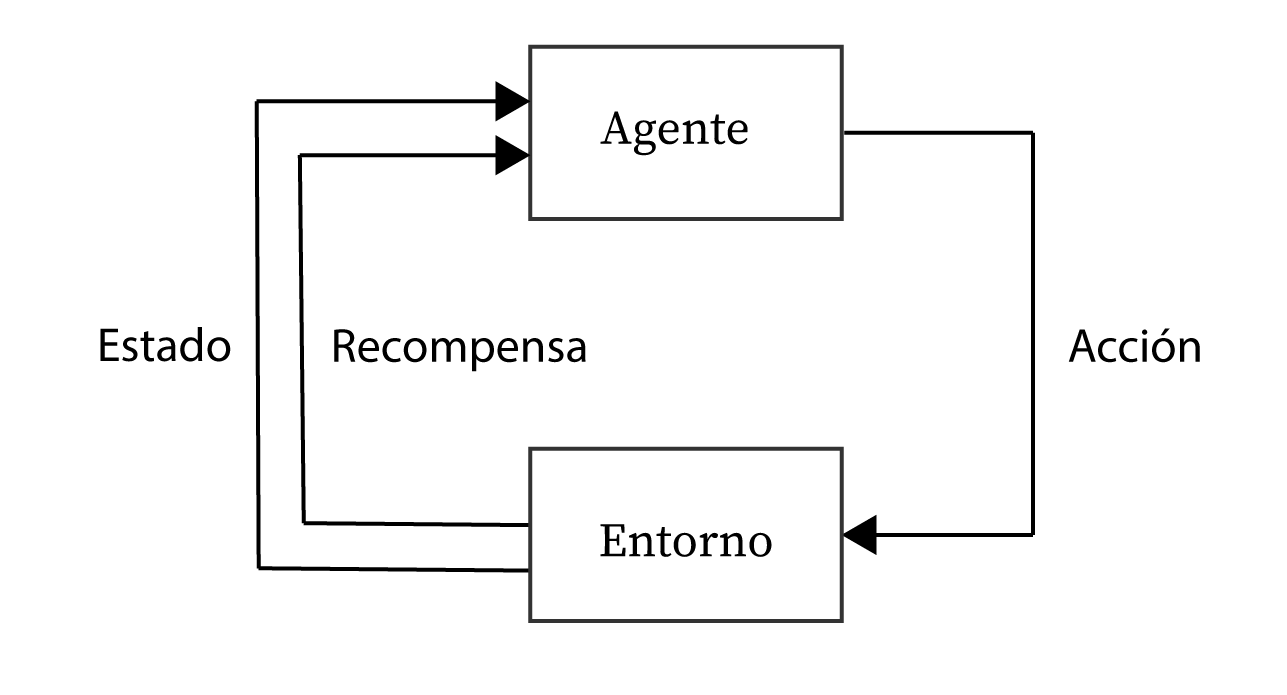
\includegraphics[width=0.7\textwidth]{Graphics/rl-elements.png}
    \caption{Diagrama de los componentes elementales del aprendizaje por refuerzo.}
    \label{fig:rl-elements}
\end{figure}

\subsection{Componentes del aprendizaje por refuerzo}

Más allá de los macroconceptos de agente, entorno, observaciones y acciones, se pueden identificar cuatro subelementos principales de un sistema de aprendizaje por refuerzo: la política, la señal de recompensa, la función de valor y, opcionalmente, el modelo del entorno. [\cite{sutton1998introduction}]

La política define la forma de actuar del agente en un momento dado. A grandes rasgos, una política es un mapeo de los estados percibidos del entorno a las acciones que se deben realizar cuando se encuentran en esos estados. La política es el núcleo de la voluntad de un agente en el sentido de que por sí sola es suficiente para determinar su comportamiento. En general, las políticas pueden ser estocásticas. [\cite{sutton1998introduction}]

La señal de recompensa define el objetivo en un problema de aprendizaje por refuerzo. En cada paso de tiempo, el entorno envía al agente de aprendizaje por refuerzo un único número, una recompensa. El único objetivo del agente es maximizar la recompensa total que recibe a largo plazo. La señal de recompensa define, pues, cuáles son los eventos buenos y malos para el agente. La recompensa enviada en cualquier momento depende de la acción del agente y el estado actual del entorno. El agente no puede alterar el proceso que lo hace. La única forma en que el agente puede influir en la señal de recompensa es a través de sus acciones, que pueden tener un efecto directo en la recompensa, o un efecto indirecto a través del cambio del estado del entorno. [\cite{sutton1998introduction}]

Las recompensas son en cierto modo primarias, mientras que los valores, como predicciones de las recompensas, son secundarios. Sin recompensas no podría haber valores, y el único propósito de estimar los valores es conseguir más recompensas. Sin embargo, son los valores los que más nos preocupan a la hora de tomar y evaluar decisiones. Las elecciones de acción se hacen en base a juicios de valor. Buscamos acciones que provoquen estados de mayor valor, no de mayor recompensa, porque estas acciones obtienen la mayor cantidad de recompensa para nosotros a largo plazo. En la toma de decisiones y la planificación, la cantidad derivada llamada valor es la que más nos preocupa. Por desgracia, es mucho más difícil determinar los valores que las recompensas. Las recompensas vienen dadas directamente por el entorno, pero los valores deben estimarse y reestimarse a partir de las secuencias de observaciones que realiza un agente a lo largo de su vida. De hecho, el componente más importante de casi todos los algoritmos de aprendizaje por refuerzo que consideramos es un método para estimar eficazmente los valores. [\cite{sutton1998introduction}] [\cite{rao2000reinforcement}]

El cuarto y último elemento de algunos sistemas de aprendizaje por refuerzo es un modelo del entorno. Se trata de algo que imita el comportamiento del entorno o, más generalmente, que permite hacer inferencias sobre cómo se comportará el entorno. Por ejemplo, dado un estado y una acción, el modelo puede predecir el siguiente estado y la siguiente recompensa resultantes. [\cite{sutton1998introduction}]


\subsection{Proceso de Decisión de Markov (MDP)}

Idealmente, es una señal de estado que resuma las sensaciones pasadas de forma compacta, pero de tal manera que se conserve toda la información relevante. Esto requiere normalmente más que las sensaciones inmediatas, pero nunca más que la historia completa de todas las sensaciones pasadas. Una señal de estado que consigue retener toda la información relevante se dice que es Markov, o que tiene la propiedad Markov. [\cite{rao2000reinforcement}] [\cite{wiering2012reinforcement}]

Siempre queremos que el estado sea una buena base para predecir futuras recompensas y para seleccionar acciones. Los estados de Markov proporcionan una base insuperable para hacer todas estas cosas. En la medida en que el estado se acerque a la capacidad de los estados de Markov en estos aspectos, se obtendrá un mejor rendimiento de los sistemas de aprendizaje por refuerzo. [\cite{wiering2012reinforcement}]

Una tarea de aprendizaje por refuerzo que satisface la propiedad de Markov se denomina Proceso de Decisión de Markov, o MDP. Si los espacios de estado y acción son finitos, se denomina Proceso de Decisión de Markov finito (MDP finito). [\cite{wiering2012reinforcement}]

La interacción agente-entorno se descompone naturalmente en una secuencia de episodios separados (tareas episódicas), y otra en la que no (tareas continuas). El primer caso es matemáticamente más fácil porque cada acción afecta sólo al número finito de recompensas recibidas posteriormente durante el episodio. [\cite{wiering2012reinforcement}]

\subsection{Principales estrategias para resolver problemas de aprendizaje por refuerzo}

El objetivo de la RL es que el agente aprenda a navegar por el entorno para maximizar una métrica de recompensa acumulada. La política es como el algoritmo que el agente perfecciona para maximizar la recompensa. Por tanto el objetivo de la RL es construir la política que máximice la recompensa acumulada, al menos de forma implícita. [\cite{sutton1998introduction}]

Los algoritmos de RL se pueden dividir utilizando varias categorizaciones, una de ellas está dada en el uso del modelo del entorno: los \textit{basados en modelos} y los \textit{libres de modelo}.

\begin{itemize}
\item Los \textit{basados en el modelo} donde el agente que intenta comprender su entorno y crear un modelo del mismo basado en sus interacciones con él. En un sistema de este tipo, las preferencias tienen prioridad sobre las consecuencias de las acciones, es decir, el agente codicioso siempre intentará realizar una acción que le permita obtener la máxima recompensa, independientemente de lo que esa acción pueda causar. Algoritmos como \textit{Dyna} son un ejemplo.

\item Por otro lado, como muestra la [Fig. \ref{fig:rl-strategies}], los algoritmos \textit{libres de modelo} buscan aprender las consecuencias de sus acciones directamente a travéz de la experiencia. En otras palabras, un algoritmo de este tipo llevará a cabo una acción varias veces y ajustará la política según sus resultados.
\end{itemize}

Si el agente puede predecir (o simular) la recompensa de una acción antes de llevarla a cabo y, por tanto, planificar lo que debe hacer, el algoritmo está basado en un modelo. Mientras que si tiene que llevar a cabo la acción, o sea una experiencia real, para ver lo que ocurre y aprender de ello, no tiene modelo.

\begin{figure}[ht!]
    \centering
    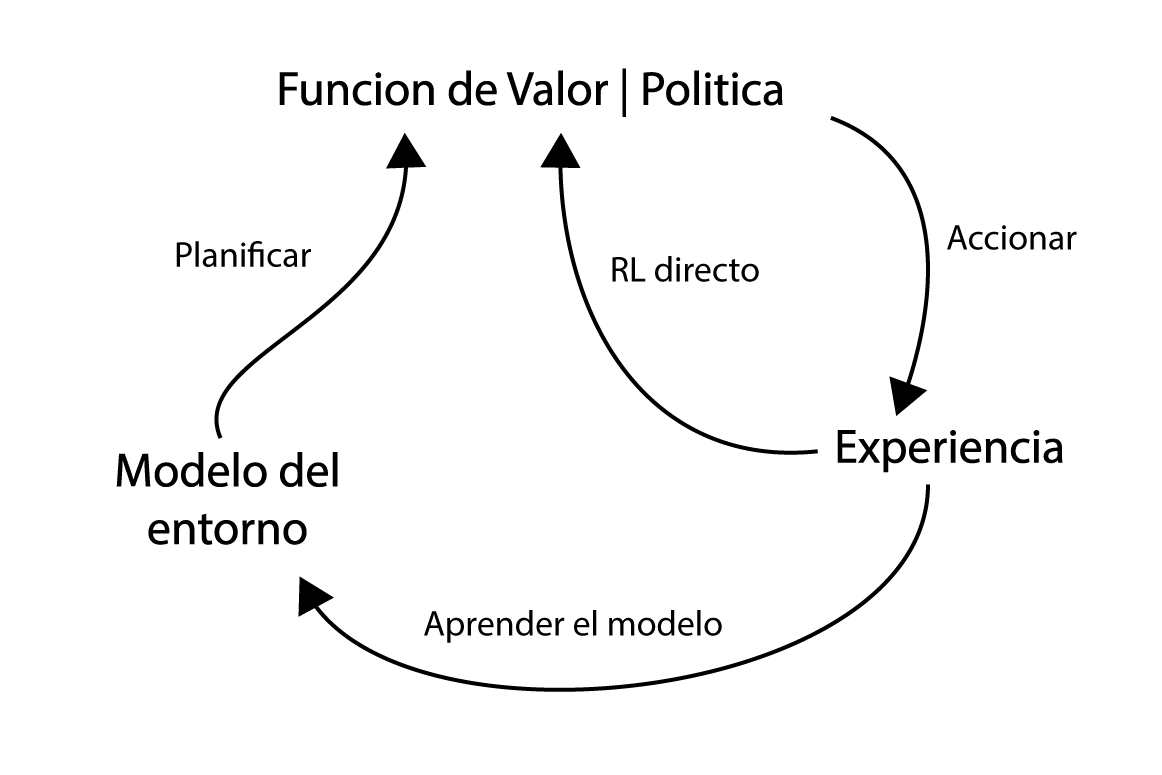
\includegraphics[width=0.7\textwidth]{Graphics/rl-strategies.png}
    \caption{Relaciones entre el aprendizaje, la planificación y la actuación.}
    \label{fig:rl-strategies}
\end{figure}


Dentro de los algoritmos  \textit{libres de modelo} existe otra caracterización basada en si se construye explicitamente o no la política del agente.

\begin{itemize}
\item En los métodos \textit{basados en políticas} se construye explícitamente una representación de una política y se mantiene en memoria durante el aprendizaje. Se puede citar los algoritmos de \textit{Policy Gradient}, \textit{Monte Carlos Tree Search}, entre otros.

\item En los métodos \textit{basados en valores} no se almancena ninguna política explícita, sólo una función de valor. La política es aquí implícita y puede derivarse directamente de la función de valor (elegir la acción con el mejor valor). Se puede citar los algoritmos de \textit{Q-Learning}, \textit{Deep Q-Learning}, \textit{SARSA}, entre otros.

\item Los algoritmos de \textit{Actor-crítico} tienen una mezcla de los dos anteriores. Se puede citar algoritmos como AlphaZero.
\end{itemize}

Los métodos on-policy intentan evaluar o mejorar la política que se utiliza para tomar las decisiones, mientras que los métodos off-policy evalúan o mejoran una política diferente a la utilizada para generar los datos. En el primer caso, el agente aprende la función de valor de la política que sigue en ese momento, mientras que en el segundo caso aprende la función de valor de la política que considera mejor en ese momento. Estas dos políticas suelen ser diferentes debido a la necesidad de explorar.

Existen otros tipos de algoritmos de aprendizaje por reforzamiento, como los geneticos o evolutivos, por imitación, entre otros; pero seran omitidos para la simplicidad del documento.

\section{Generalizacion en machine learning}\label{section:state-of-the-art:generalization-on-machine-learning}

La generalización es la capacidad de manejar situaciones (o tareas) que difieren de las situaciones anteriores. En inteligencia artificial se caracteriza como el rendimiento de un modelo en entradas que no formaban parte de sus datos de entrenamiento.

La capacidad generalización se basa fundamentalmente en las nociones relacionadas a la novedad e incertidumbre. Un sistema sólo puede generalizar ante información nueva que no pueda ser conocida de antemano ni por el sistema o por su creador. Dicha capacidad puede se pone en evidencia a medida que aumenta el dominio de las tareas y problemas que se pueden manejar. Para entender mejor estas nociones se definirán varios conceptos a continuación.

\subsection{Tipos de Generalizacion}

\begin{itemize}
\item \textit{Generalización centrada en el sistema:} es la capacidad de un sistema de aprendizaje para manejar situaciones que no ha encontrado antes. La noción formal de error de generalización en la teoría del aprendizaje estadístico pertenecería aquí.

\item \textit{Generalización consciente del desarrollador:} es la capacidad de un sistema, ya sea de aprendizaje o estático, para manejar situaciones que ni el sistema ni el desarrollador del sistema han encontrado antes.
\end{itemize}


\subsection{Grados de Generalizacion}

Aunque los límites entre los grados de la escala de generalización son mayormente difusos y continuos, se ha agrupado en 4 niveles fundamentales de interés para el estudio:

\begin{itemize}
\item \textit{Ausencia de generalización:} Los sistemas de IA en los que no hay incertidumbre no muestran generalización. Por ejemplo, no se puede decir que un programa que juega a "4 en Línea" mediante una iteración exhaustiva "generalice" a todas las configuraciones del tablero.

\item \textit{Generalización local o robustez:} Es la capacidad de un sistema para manejar nuevos puntos de una distribución conocida para una sola tarea o un conjunto bien delimitado de tareas conocidas, dado un muestreo suficientemente denso de ejemplos de la distribución (por ejemplo, la tolerancia a las perturbaciones previstas dentro de un contexto fijo). Por ejemplo, se puede decir que un clasificador de imágenes que puede distinguir imágenes RGB de 150x150 no vistas anteriormente que contienen gatos de las que contienen perros, después de haber sido entrenado con muchas de esas imágenes etiquetadas, realiza una generalización local. 

\item \textit{Generalización amplia o flexibilidad:} Es la capacidad de un sistema para manejar una amplia categoría de tareas y entornos sin más intervención humana. Esto incluye la capacidad de manejar situaciones que no podrían haber sido previstas por los creadores del sistema. Podría considerarse que refleja la capacidad del ser humano en un único y amplio ámbito de actividad (por ejemplo, las tareas domésticas o la conducción en el mundo real).

\item \textit{Generalización extrema:} Describe los sistemas abiertos con la capacidad de abordar tareas completamente nuevas que sólo comparten puntos comunes abstractos con situaciones previamente encontradas, aplicables a cualquier tarea y dominio dentro de un amplio alcance. Esto podría caracterizarse como "adaptación a incógnitas desconocidas en una gama desconocida de tareas y dominios". Las formas biológicas de inteligencia (los humanos y posiblemente otras especies in- telligentes) son el único ejemplo de un sistema de este tipo en este momento.
\end{itemize}

A esta lista podríamos, en teoría, añadir una entrada más: \textit{La universalidad}, que extendería la generalidad" más allá del ámbito de las tareas relevantes para los humanos, a cualquier tarea que pueda ser abordada de forma práctica dentro de nuestro universo (nótese que esto es diferente de cualquier tarea en absoluto, tal y como se entiende en los supuestos del teorema \textit{No Free Lunch}).

Es importante destacar que el espectro de la generalización descrito anteriormente parece reflejar la organización de las capacidades cognitivas de los seres humanos tal y como se establece en las teorías de la estructura de la inteligencia en la psicología cognitiva donde se define el \textit{factor g} como una razón global y presente en el nivel de inteligencia del hombre. 

\begin{figure}[ht!]
    \centering
    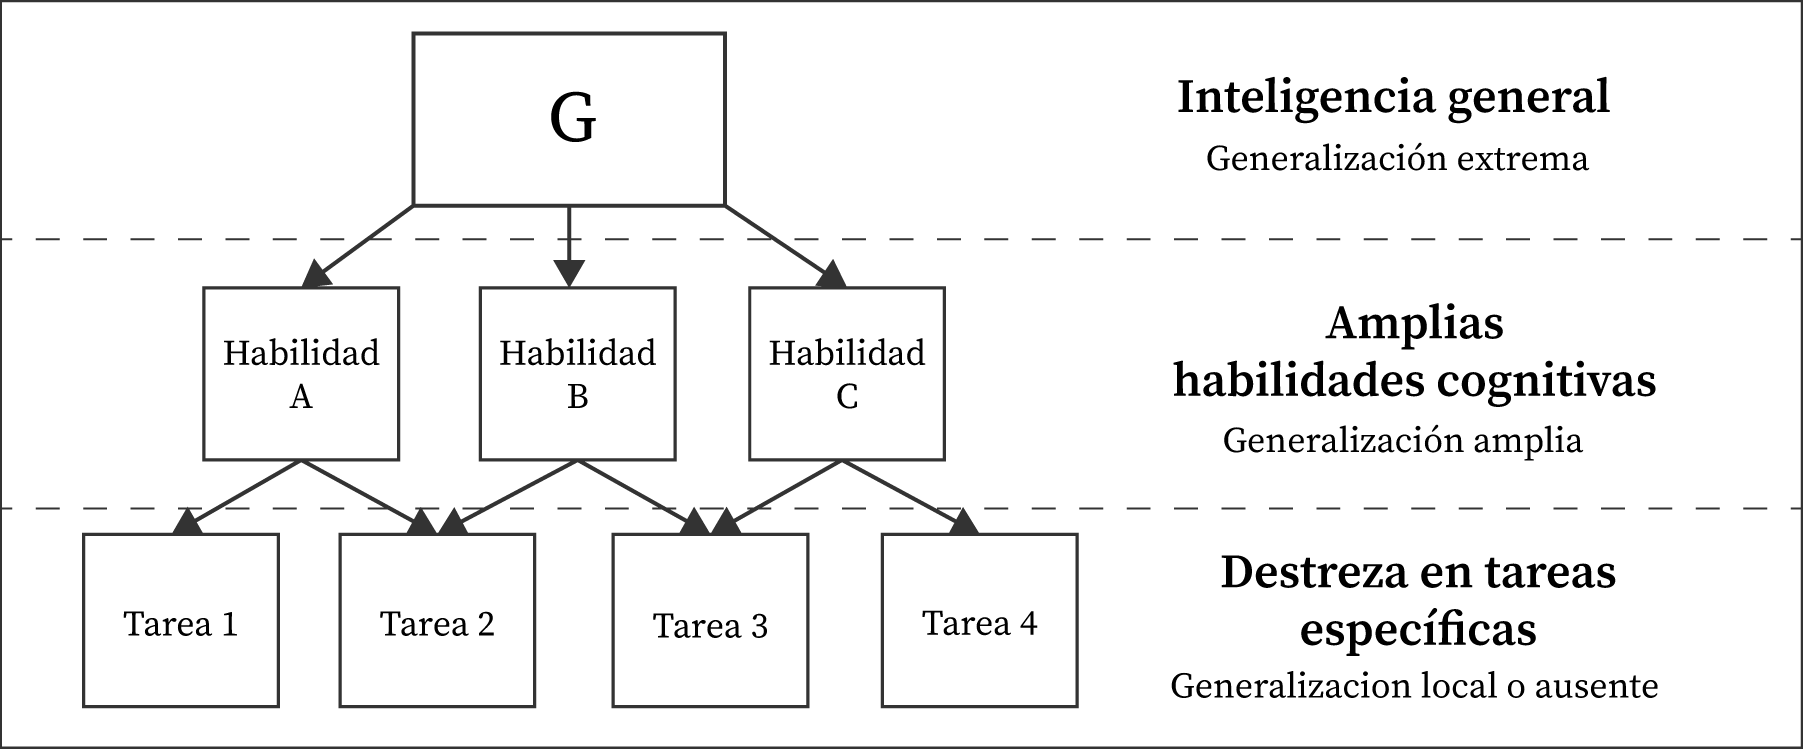
\includegraphics[width=0.7\textwidth]{Graphics/g-factor.png}
    \caption{Modelo jerárquico de las capacidades cognitivas y su correspondencia con el espectro de la generalización.}
    \label{fig:g-factor}
\end{figure}

\section{Evaluación de algoritmos}\label{section:state-of-the-art:evaluating-algoritms}

Las medidas de rendimiento que cuantifican la habilidad de un sistema en una tarea determinada han impulsado el exito de la inteligencia artificial. No existe una forma única y formalizada de realizar una evaluación basada en la destreza. Entre los enfoques que han tenido éxito históricamente se encuentran:

\begin{itemize}
\item Revision humana: Hacer que jueces humanos observen la respuesta de entrada-salida del sistema y la puntúen. Esta es la idea que subyace al test de Turing y sus variantes. Este modo de evaluación rara vez se utiliza en la práctica, debido a que es caro, imposible de automatizar y subjetivo. Algunos sistemas de IA orientados al ser humano (en particular los chatbots comerciales) lo utilizan como uno de los múltiples mecanismos de evaluación.

\item Analisis en Caja-Blanca (White-Box Analysis): Inspeccionar la implementación del sistema para determinar su respuesta de entrada-salida y puntuarla. Esto es más relevante para los algoritmos que resuelven una tarea totalmente descrita en un entorno totalmente descrito en el que todas las entradas posibles pueden enumerarse explícitamente o describirse analíticamente y a menudo tomaría la forma de una prueba de optimalidad.

\item Oponencial (Peer Confrontation): Hacer que el sistema compita contra otras IAs o contra humanos. Este es el modo de evaluación preferido para los juegos de jugador contra jugador, como el ajedrez.

\item Comparaciones de referencia (Benchmarks): Hacer que el sistema produzca resultados para un conjunto de pruebas de entradas (o entornos) para los que se conoce el resultado deseado, y puntuar la respuesta.
\end{itemize}

Los \textit{Benchmarks}, en particular, han sido un importante motor de progreso en la IA, porque son reproducibles (el conjunto de pruebas es fijo), justos (el conjunto de pruebas es el mismo para todos), escalables (es barato realizar la evaluación muchas veces), fáciles de configurar y lo suficientemente flexibles como para ser aplicables a una amplia gama de tareas posibles. Los puntos de referencia han sido a menudo más impactantes en el contexto de una competición entre diferentes equipos de investigación.

La robustez de los sistemas que se desarrollan, en particular los modelos de Deep Learning, suele ser problemática. Esto se debe en gran parte al hecho de que la mayoría de los benchmarks no prestan mucha atención a la evaluación formal de la robustez y a la cuantificación de la generalización, y por lo tanto pueden ser resueltos a través de atajos que el descenso de gradiente es apto para explotar. La generalización entre tareas sigue siendo difícil para los algoritmos de aprendizaje profundo por refuerzo más avanzados. Aunque los agentes entrenados pueden resolver tareas complejas, les cuesta transferir su experiencia a nuevos entornos. Los agentes que dominan diez niveles de un videojuego suelen fracasar estrepitosamente cuando se enfrentan por primera vez al undécimo. Los humanos pueden generalizar sin problemas en tareas similares, pero esta capacidad está ausente en los agentes de la realidad virtual. En resumen, los agentes se especializan demasiado en los entornos encontrados durante el entrenamiento [\cite{cobbe2019quantifying}]. A este fenómeno se le denomina sobre  \textit{overfitting}. Se reconoce ampliamente que los agentes de RL son propensos a la sobreadaptación [\cite{zhang2018study}], pero los puntos de referencia de RL más comunes siguen fomentando el entrenamiento y la evaluación en el mismo conjunto de entornos. [\cite{nichol2018gotta}] 

\section{Una buena evaluacion de Inteligencia}\label{section:state-of-the-art:a-good-measure-of-inteligence}

La base de la inteligencia. Los prejuicios y las experiencias.

Tipos de prejuicios y experiencias a considerar:
- **Premisas de bajo nivel**: Conocimientos sobre nuestro propio espacio sensoriomotor. Reflejos e instintos inatos.
- **Premisas de metaaprendizaje**: Rigen nuestras estrategias de aprendizaje y capacidades de adquisición de conocimientos.
- **Conocimientos previos de alto nivel**: Conocimientos sobre los objetos y fenómenos de nuestro entorno externo.

Las premisas de metraaprendizaje son objetivo de esta ciencia. Es la inteligencia en si misma. Entender como el cerebro transforma experiencias en conocimientos y habilidades.

La comparación entre dos sistemas debe ser JUSTA teniendo en cuenta los **Conocimientos previos de alto nivel** que posean. 


Tambien debe considerarse el **Ambito de tareas compartido** entre los sistemas a comparar. Y el grado de especializacion que son alcanzables en ese ambito.

Caracteristicas necesarias para una evaluacion de inteligencia extrema:
- Debe describir el Ambito de la evaluacion
- Replicable o Repoducible.
- No debe limitase a la habilidad en una tarea.
- Debe contener tareas no conocidas por los desarrolladores.
- Controlar la cantidad de experiencia que se brinda.
- Definir el conjunto de premisas de Conocimiento previo.
- Deberia funcionar para humanos y maquinas.
- Debe justificar la dificultad de generalizacion

\section{Entornos de evaluacion de Inteligencia}\label{section:state-of-the-art:inteligence-evaluation-enviroments}

\subsection{Primeras pruebas propuestas}

Las primeras ideas para evaluacion eran por Revision humana y tenian un caracter Antropocéntrico.

\subsubsection{Juego de Imitación}
% - **Juego de Imitación** (Test de Turing), explicacion.

\subsubsection{Prueba del Café}
% - **Prueba del Café**, explicacion.

\subsubsection{Pruebas psicometricas}
% - **Pruebas psicometricas**, explicacion.

Comentar sobre la inefectividad y los problemas que trae hacer evaluaciones con supervision. (Mencionar las buenas practicas para evaluaciones de mas adelante)

\subsection{Otas propuestas de evaluación}

La actual tendencia de investigadores por desarrollar algoritmos de proposito general.  

Ejemplos de algunas evaluaciones mas modernas pero no se implementaron.

\subsubsection{The bica cognitive decathlon (2004)}

\subsubsection{Olimpiadas de Turing (2014)}

[\cite{beyret2019animal}]


\subsection{Entornos de evaluación con tareas conocidas}\label{section:state-of-the-art:inteligence-evaluation-enviroments:evaluation-enviroments-with-know-tasks}

Por lo general utilizan amplias baterías de tareas de prueba para evaluar sistemas que buscan una mayor flexibilidad. En estos entornos los desarrolladores del sistema evaluado conocen de antemano el tipo de tareas que enfrentarán, solo que los escenarios varian tantos que resolver dichas tareas requerirán diferentes formas de "razonamiento" y "creatividad", expresion directa de la generalización a partir de su entrenamiento.

La lógica subyacente de estos esfuerzos es medir algo más general que la habilidad en una tarea específica ampliando el conjunto de tareas objetivo. Sin embargo, cuando se trata de evaluar la flexibilidad, un defecto crítico de estos puntos de referencia multitarea es que el conjunto de tareas sigue siendo conocido de antemano por los desarrolladores de cualquier sistema de realización de pruebas, y se espera que los sistemas de realización de pruebas sean capaces de practicar específicamente para las tareas objetivo, aprovechar el conocimiento previo incorporado específico de la tarea heredado de los desarrolladores del sistema, aprovechar el conocimiento externo obtenido a través del preentrenamiento, etc.

Medir únicamente la destreza en una tarea determinada no es suficiente para medir la inteligencia, porque la destreza está fuertemente modulada por el conocimiento previo y la experiencia: los datos de entrenamiento ilimitados permiten a los experimentadores "comprar" niveles arbitrarios de destreza para un sistema, de forma que se enmascara el propio poder de generalización del sistema.
- citar openIA con sus sistemas para jugar Dota etc

\section{Entornos de evaluacion de la capacidad de generalizacion en algoritmos RL}\label{section:state-of-the-art:evaluation-enviroments-for-generalization-on-rl-algoritms}

Los entornos de evaluacion para RL, en su mayoria se enfocan en la generalicacion local o flexible.

\subsection{The Arcade Learning Environment}\label{section:state-of-the-art:evaluation-enviroments-for-generalization-on-rl-algoritms:ALE}

ALE está construido sobre Stella1 , un emulador de Atari 2600 de código abierto. Permite al usuario interactuar con la Atari 2600 recibiendo los movimientos del joystick, enviando información de la pantalla y/o de la RAM, y emulando la plataforma. ALE también proporciona una capa de manejo de juegos que transforma cada juego en un problema estándar de aprendizaje por refuerzo, identificando la puntuación acumulada y si el juego ha terminado. Por defecto, cada observación consiste en una única pantalla de juego (frame): una matriz 2D de píxeles de 7 bits, de 160 píxeles de ancho por 210 de alto. El espacio de acción está formado por las 18 acciones discretas definidas por el mando del joystick. La capa de gestión del juego también especifica el conjunto mínimo de acciones necesarias para jugar a un determinado juego, aunque ninguno de los resultados de este artículo hace uso de esta información. Cuando se ejecuta en tiempo real, el simulador genera 60 fotogramas por segundo, y a toda velocidad emula hasta 6000 fotogramas por segundo. La recompensa en cada paso de tiempo se define juego por juego, normalmente tomando la diferencia de puntuación o puntos entre fotogramas. Un episodio comienza en el primer fotograma después de que se emita un comando de reinicio, y termina cuando el juego termina. La capa de gestión del juego también ofrece la posibilidad de terminar el episodio después de un número predefinido de fotogramas. Por lo tanto, el usuario tiene acceso a varias docenas de juegos a través de una única interfaz común, y añadir soporte para nuevos juegos es relativamente sencillo. [\cite{bellemare2013arcade}]

\begin{figure}[ht!]
    \centering
    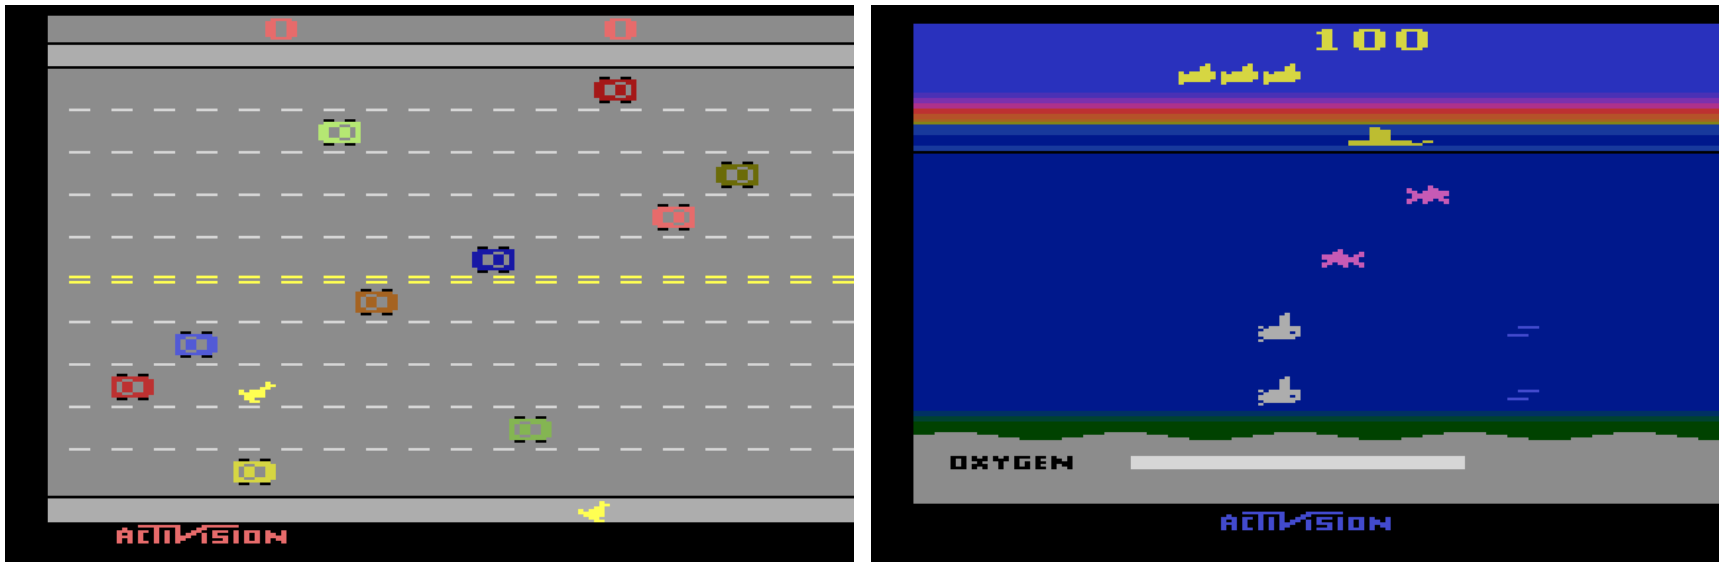
\includegraphics[width=0.7\textwidth]{Graphics/ale.png}
    \caption{Capturas de pantalla de varios juegos de ALE}
    \label{fig:ale}
\end{figure}

En [\cite{farebrother2018generalization}] también se aborda este problema, reconociendo activamente que la confusión de los entornos de entrenamiento y prueba ha contribuido a la falta de regularización en la RL profunda. Proponen utilizar diferentes modos de juego de Atari 2600 para medir la generalización. Recurren al aprendizaje supervisado en busca de inspiración, descubriendo que tanto la regularización L2 [\cite{krogh1991simple}] como el abandono pueden ayudar a los agentes a aprender características más generables.

Desde el ajedrez [\cite{silver2017mastering}] hasta el Go [\cite{silver2016mastering}], desde los antiguos juegos de Atari [\cite{bellemare2013arcade}] hasta Star- craft 2 [\cite{vinyals2017starcraft}], se ve una gran variedad de entornos desafiantes en los que la IA supera ahora a los humanos. Éxitos como estos en el aprendizaje por refuerzo incluso han dado lugar a la transferencia de agentes entrenados al mundo real para manipulaciones robóticas [\cite{andrychowicz2020learning}]. Estos impresionantes resultados son solo un primer paso hacia agentes que puedan interactuar de forma robusta con sus entornos. En estos entornos, la mayoría de las tareas utilizadas para el entrenamiento son idénticas, o extremadamente similares, a las utilizadas para las pruebas. Aunque el agente no siempre ha estado expuesto a las tareas de prueba durante el entrenamiento, probablemente ha estado expuesto a tareas extraídas de la misma distribución. Esto da lugar a agentes que alcanzan un rendimiento sobrehumano en problemas específicos, pero que son incapaces de generalizar [\cite{packer2018assessing}].

\subsection{CoinRun}

El entorno CoinRun tiene como proposito evaluar el rendimiento de la genalización de los agentes. El objetivo de cada nivel de CoinRun es sencillo: recoger la única moneda que se encuentra al final del nivel. El agente controla un personaje que aparece en el extremo izquierdo y la moneda aparece en el extremo derecho. Entre el agente y la moneda hay varios obstáculos, tanto fijos como no fijos. La colisión con un obstáculo provoca la muerte inmediata del agente. La única recompensa en el entorno se obtiene al recoger la moneda, y esta recompensa es una constante positiva fija. El nivel termina cuando el agente muere, se recoge la moneda o después de 1000 pasos de tiempo [\cite{cobbe2019quantifying}].

\begin{figure}[ht!]
    \begin{subfigure}
      \centering
      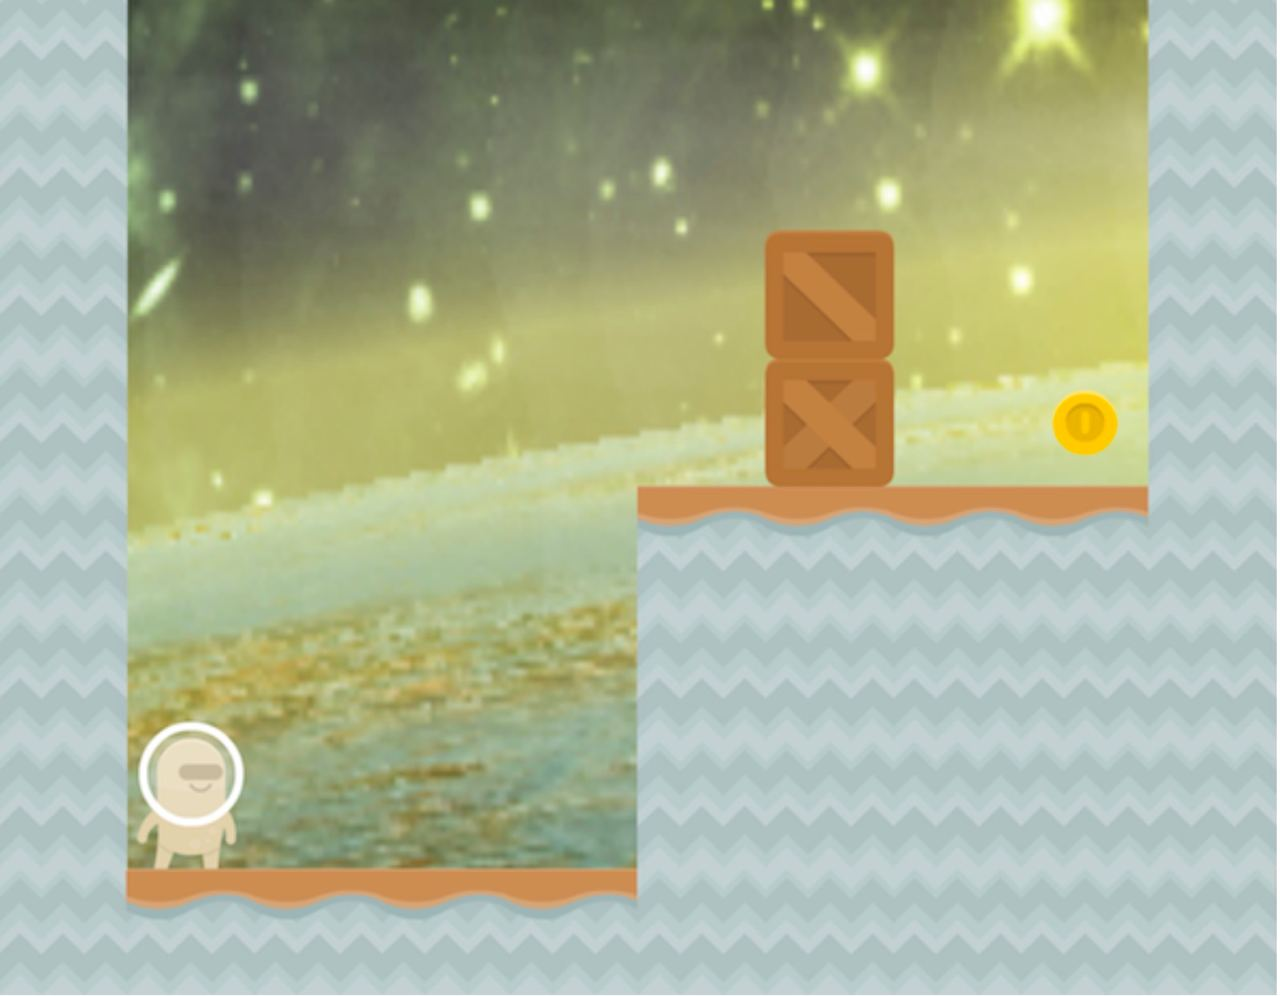
\includegraphics[width=0.5\textwidth]{Graphics/coinrun_1.jpeg}
      \label{fig:coinrun1}
    \end{subfigure}%
    \begin{subfigure}
      \centering
      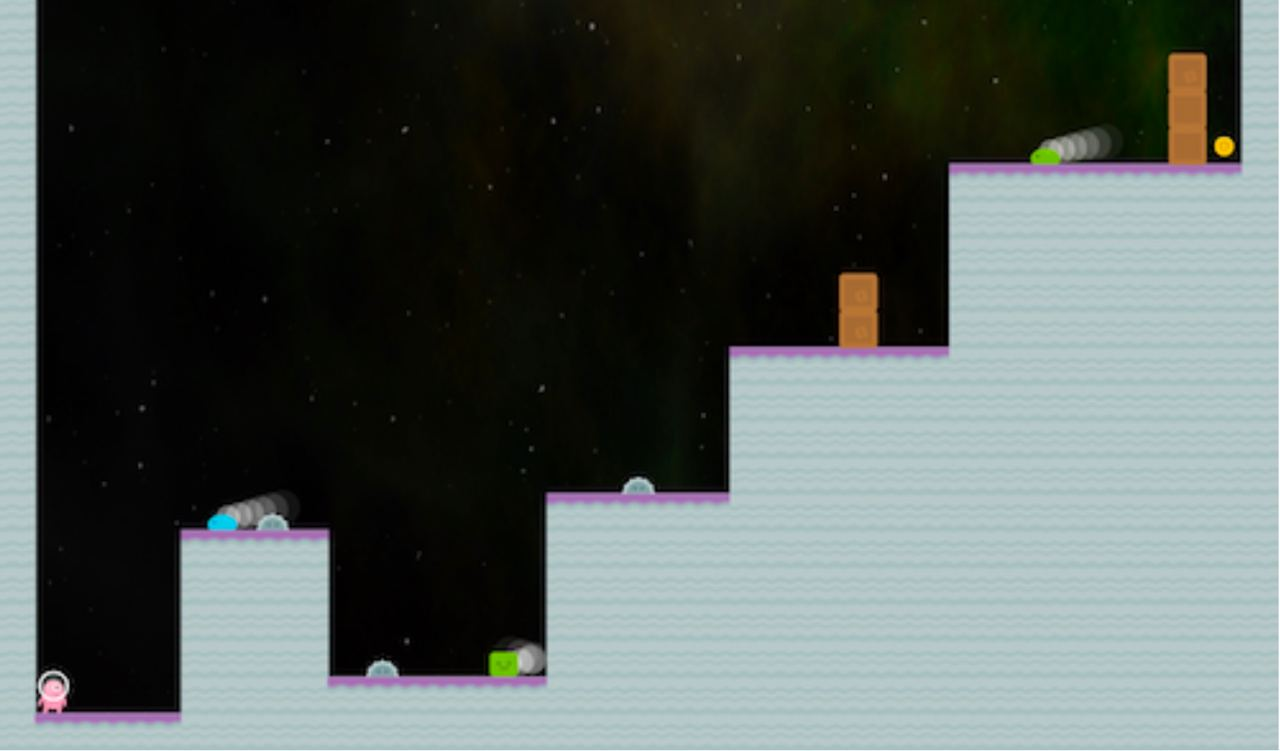
\includegraphics[width=0.5\textwidth]{Graphics/coinrun_2.jpeg}
      \label{fig:coinrun2}
    \end{subfigure}%
    \caption{Niveles de CoinRun con diferente dificultad}
    \label{fig:coinrun}
\end{figure}

El juego CoinRun esta diseñado para que sea manejable para los algoritmos existentes. Es decir, dado un número suficiente de niveles de entrenamiento y un tiempo de entrenamiento suficiente, nuestros algoritmos aprenden una política casi óptima para todos los niveles de CoinRun. Cada nivel se genera de forma determinista a partir de una semilla dada, lo que proporciona a los agentes acceso a un suministro de datos de entrenamiento arbitrariamente grande y fácilmente cuantificable. CoinRun imita el estilo de juegos como Sonic [\cite{nichol2018gotta}], pero es mucho más sencillo. Para evaluar la generalización, esta simplicidad puede ser muy ventajosa. Los niveles varían mucho en dificultad, por lo que su distribución y organización forma naturalmente un plan de estudios para el agente [\cite{cobbe2019quantifying}].

CoinRun está diseñado para ser lo suficientemente simple como para que los niveles individuales sean fáciles de resolver cuando se entrena, pero la tarea es crear un agente que pueda resolver variaciones no vistas. La generación procedural de niveles y organización de dificultad tiene un efecto positivo en la evaluación de la generalización apoyada por la unión a las técnicas sugeridas para evitar sobreajuste en el entrenamiento. No definir explicitamente las premisas de conocimiento que deberian poseer los agentes para ser evaluados y la simplicidad de las tareas impiden su uso como prueba para niveles de generalizacion mas amplios.

\subsection{Procgen}

Procgen Benchmark consta de 16 entornos únicos diseñados por sus creadores e inspirados por [\cite{bellemare2013arcade}] para medir tanto la eficiencia de las muestras como la generalización en el aprendizaje por refuerzo. Estos entornos se benefician en gran medida del uso de la generación de contenido proceduralmente, la creación algorítmica de un suministro casi infinito de contenido altamente dominado. En estos entornos, emplear la generación procedural es mucho más eficaz que confiar en contenidos fijos diseñados por el ser humano. [\cite{cobbe2020leveraging}]

La lógica de generación procedural rige el diseño de los niveles, la selección de los recursos del juego, la ubicación y los tiempos de aparición de las entidades, y otros detalles específicos del juego. Para dominar cualquiera de estos entornos, los agentes deben aprender una política que sea robusta en todos los ejes de variación [\cite{cobbe2020leveraging}]. El aprendizaje de una política de este tipo es más desafiante y más relevante que el ajuste excesivo a un puñado de niveles fijos, como en el caso de ALE visto en \ref{section:state-of-the-art:evaluation-enviroments-for-generalization-on-rl-algoritms:ALE}. 

Para facilitar la ejecución Procgen presenta un espacio fijo de observaciones y acciones. Contando observaciones de tamaño $64*64*3(RGB)$ y $15$ acciones posibles, donde cada entorno define cuales de estas son aplicables. [\cite{cobbe2020leveraging}]

Las cualidades de Procgen le permiten crear entornos para probar diferentes caracteristicas de algoritmos de aprendizaje por reforzamiento, tales como la exploración, capacidad de memoria, y generalizacion local.

Otro ejemplo similar, \textbf{Obstacle Tower} [\cite{juliani2019obstacle}] es un nuevo juego en 3D basado en la venganza de Moctezuma, uno de los juegos Atari más difíciles (para la IA), cuyas fases se generan de forma procedural. 

\begin{figure}[ht!]
    \centering
    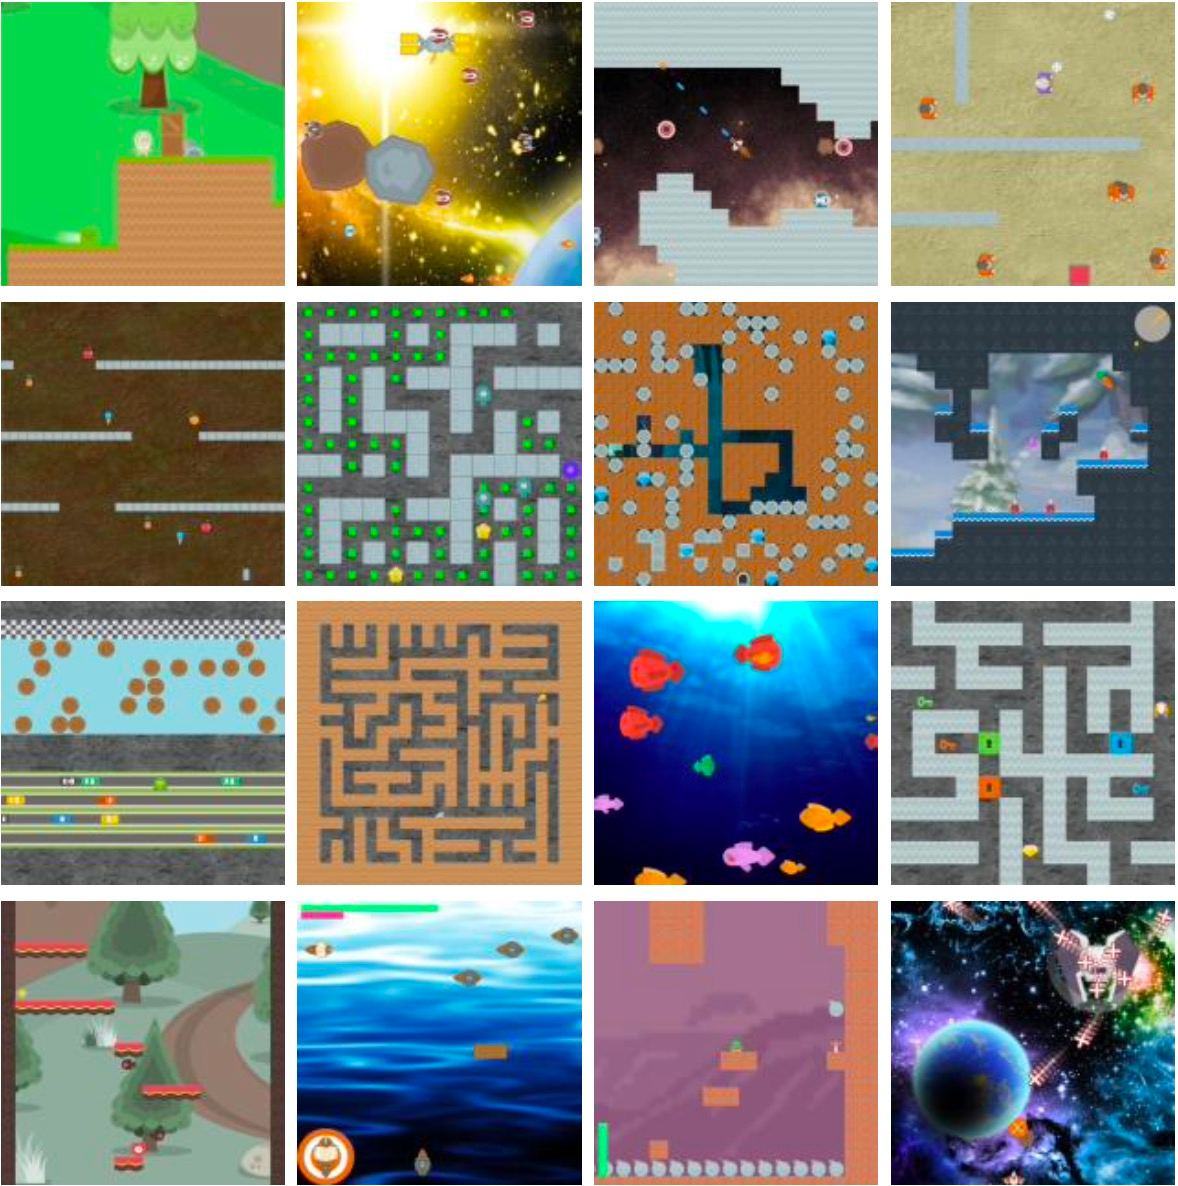
\includegraphics[width=0.7\textwidth]{Graphics/procgen.jpeg}
    \caption{Capturas de pantalla de varios juegos de Procgen}
    \label{fig:procgen}
\end{figure}

\subsection{The Animal-AI Environment}


\section{Project Malmo, un meta-entorno de pruebas en Minecraft}\label{section:state-of-the-art:project-malmO}

Ambito de evaluacion.

Premisas implicitas de conocimiento.

\subsection{MineRL y la prueba del Diamante}

Esta ambiciosa competición está diseñada para impulsar los avances en el aprendizaje de refuerzo con muestras eficientes y con prejuicios humanos. El aprendizaje eficiente por muestreo es un reto clave, ya que los algoritmos actuales suelen requerir millones de muestras para aprender a realizar tareas concretas, lo que limita el alcance y la aplicabilidad de estos enfoques. Esta competición se basa en una tarea compleja, en datos de demostración a gran escala y en una configuración de evaluación que requiere y premia el aprendizaje eficiente de las muestras y la generalización efectiva. [\cite{hofmann2019minecraft}]

Comparando entre la inteligencia artificial y las capacidades mentales de un niño de siete años, apoyándonos en el popular videojuego Minecraft, donde dicho humano puede aprender a encontrar un diamante raro en el juego tras ver una rápida demostración en YouTube. La inteligencia artificial (IA) estaría lejos de logarlo de esta forma. Pero a través de una competición informática los investigadores esperan reducir la distancia entre la máquina y el niño y, de este modo, se reduciría la potencia de cálculo necesaria para entrenar a las IA.
Los competidores pueden tardar hasta cuatro días y utilizar no más de ocho millones de pasos para entrenar a sus IA a encontrar un diamante. Eso es mucho más tiempo del que tardaría un niño en aprender, pero mucho más rápido que los modelos típicos de IA de hoy en día.

El concurso está diseñado para estimular los avances del aprendizaje por imitación que contrasta con la técnica de aprendizaje por refuerzo. El concurso se centra en el uso de la imitación para arrancar el aprendizaje, de modo que las IA no tengan que dedicar tanto tiempo a explorar el entorno para averiguar lo que es posible a partir de los primeros principios, y en su lugar utilicen los conocimientos que los humanos han acumulado. 

Para llegar al tesoro del diamante, los jugadores controlados por la IA, o agentes, en el concurso MineRL tienen que dominar un proceso de varios pasos. Primero, recogen madera y hierro para fabricar picos. Luego construyen antorchas para iluminar el camino. También pueden llevar un cubo de agua para apagar las corrientes de lava subterráneas. Una vez preparado todo eso, una IA puede empezar a explorar pozos mineros y cuevas, así como a hacer túneles bajo tierra para buscar mineral de diamante.

Para crear datos de entrenamiento para la competición, los organizadores de MineRL crearon un servidor público de Minecraft y reclutaron a personas para que completaran retos diseñados para demostrar tareas específicas, como la elaboración de diversas herramientas. Al final, capturaron 60 millones de ejemplos de acciones que podían realizarse en una situación determinada y aproximadamente 1.000 horas de comportamiento grabado para entregar a los equipos. Las grabaciones representan uno de los primeros y mayores conjuntos de datos dedicados específicamente a la investigación del aprendizaje por imitación.

Puntos fuertes y debiles según nuestra definición.

Posibles aplicaciones.



\section{Abstraction and Reasoning Corpus (ARC)}\label{section:state-of-the-art:arc}

Descripcion. Objetivos.

Ambito de evaluacion.

Descripcion de premisas de conocimientos.

Puntos débiles

Resumen y dar paso a la solucion que proponemos.

ARC tiene muchos buenos aspectos para destacar, y cumple con un gran número caracteristicas de un buen evaluador de inteligencia. Aún así su ambito de habilidad se centra en sistemas inteligentes státicos de entrada-salida, sin oportunidad de interacción. Las tareas se crean manualmente por lo que son fijas, no generativas. También se hace complejo evaluar a los algoritmos de aprendizaje por reforzamiento dado la forma en que está diseñada la prueba. Las tareas de proposito general capturadas en ARC carecen del concepto de tiempo. Las nociones de topología se deben dar de forma implícita. 



Es necesario y mas justo replantear las premisas teniendo en cuenta el efecto del tiempo, la persepcion explicita de los cambios topograficos y los efectos acción-reacción. Llevar las tareas a conceptos mas primitivos en terminos de aprendizaje sin descuidar la dificultad de generalizacion.